\chapter{Analisis}
\label{chap:analisis}

Pada bab ini akan dijelaskan analisis tentang aplikasi sejenis yang menggunakan \textit{smartphone} sebagai pengendali permainan berbasis web.

\section{AirConsole}
\label{sec:AirConsole}

Salah satu aplikasi sejenis permainan berbasis web dengan memanfaatkan \textit{smartphone} sebagai pengendali yaitu AirConsole. Aplikasi tersebut memanfaatkan teknologi \textit{browser}, \textit{smartphone}, \textit{PC}, dan juga jaringan internet untuk dapat menggunakannya. Aplikasi ini dikembangkan oleh N-Dream AG.

\textbf{Analisis AirConsole} 

AirConsole merupakan permainan berbasis web dimana \textit{browser} pada \textit{mobile device} dapat melakukan koneksi ke \textit{browser} pada  \textit{PC}. Pada aplikasi ini, terdapat berbagai macam permainan yang dapat dipilih oleh pemain. Untuk dapat memainkan aplikasi tersebut, pemain harus membuka alamat web \textit{airconsole.com} pada \textit{PC browser} dan juga pada \textit{smartphone browser}.

Analisis dilakukan dengan cara berikut:
\begin{enumerate}
	\item Memainkan permainan dari awal hingga akhir.
	\item Keluar dari \textit{browser} pada \textit{PC} pada saat permainan berlangsung.
	\item Keluar dari \textit{browser} pada \textit{smartphone} pada saat permainan berlangsung.
\end{enumerate}
Pada halaman awal web di \textit{PC}, pemain diminta untuk menekan tombol \textit{start} yang ada pada gambar berikut: 

\begin{figure}[H]
	\centering
	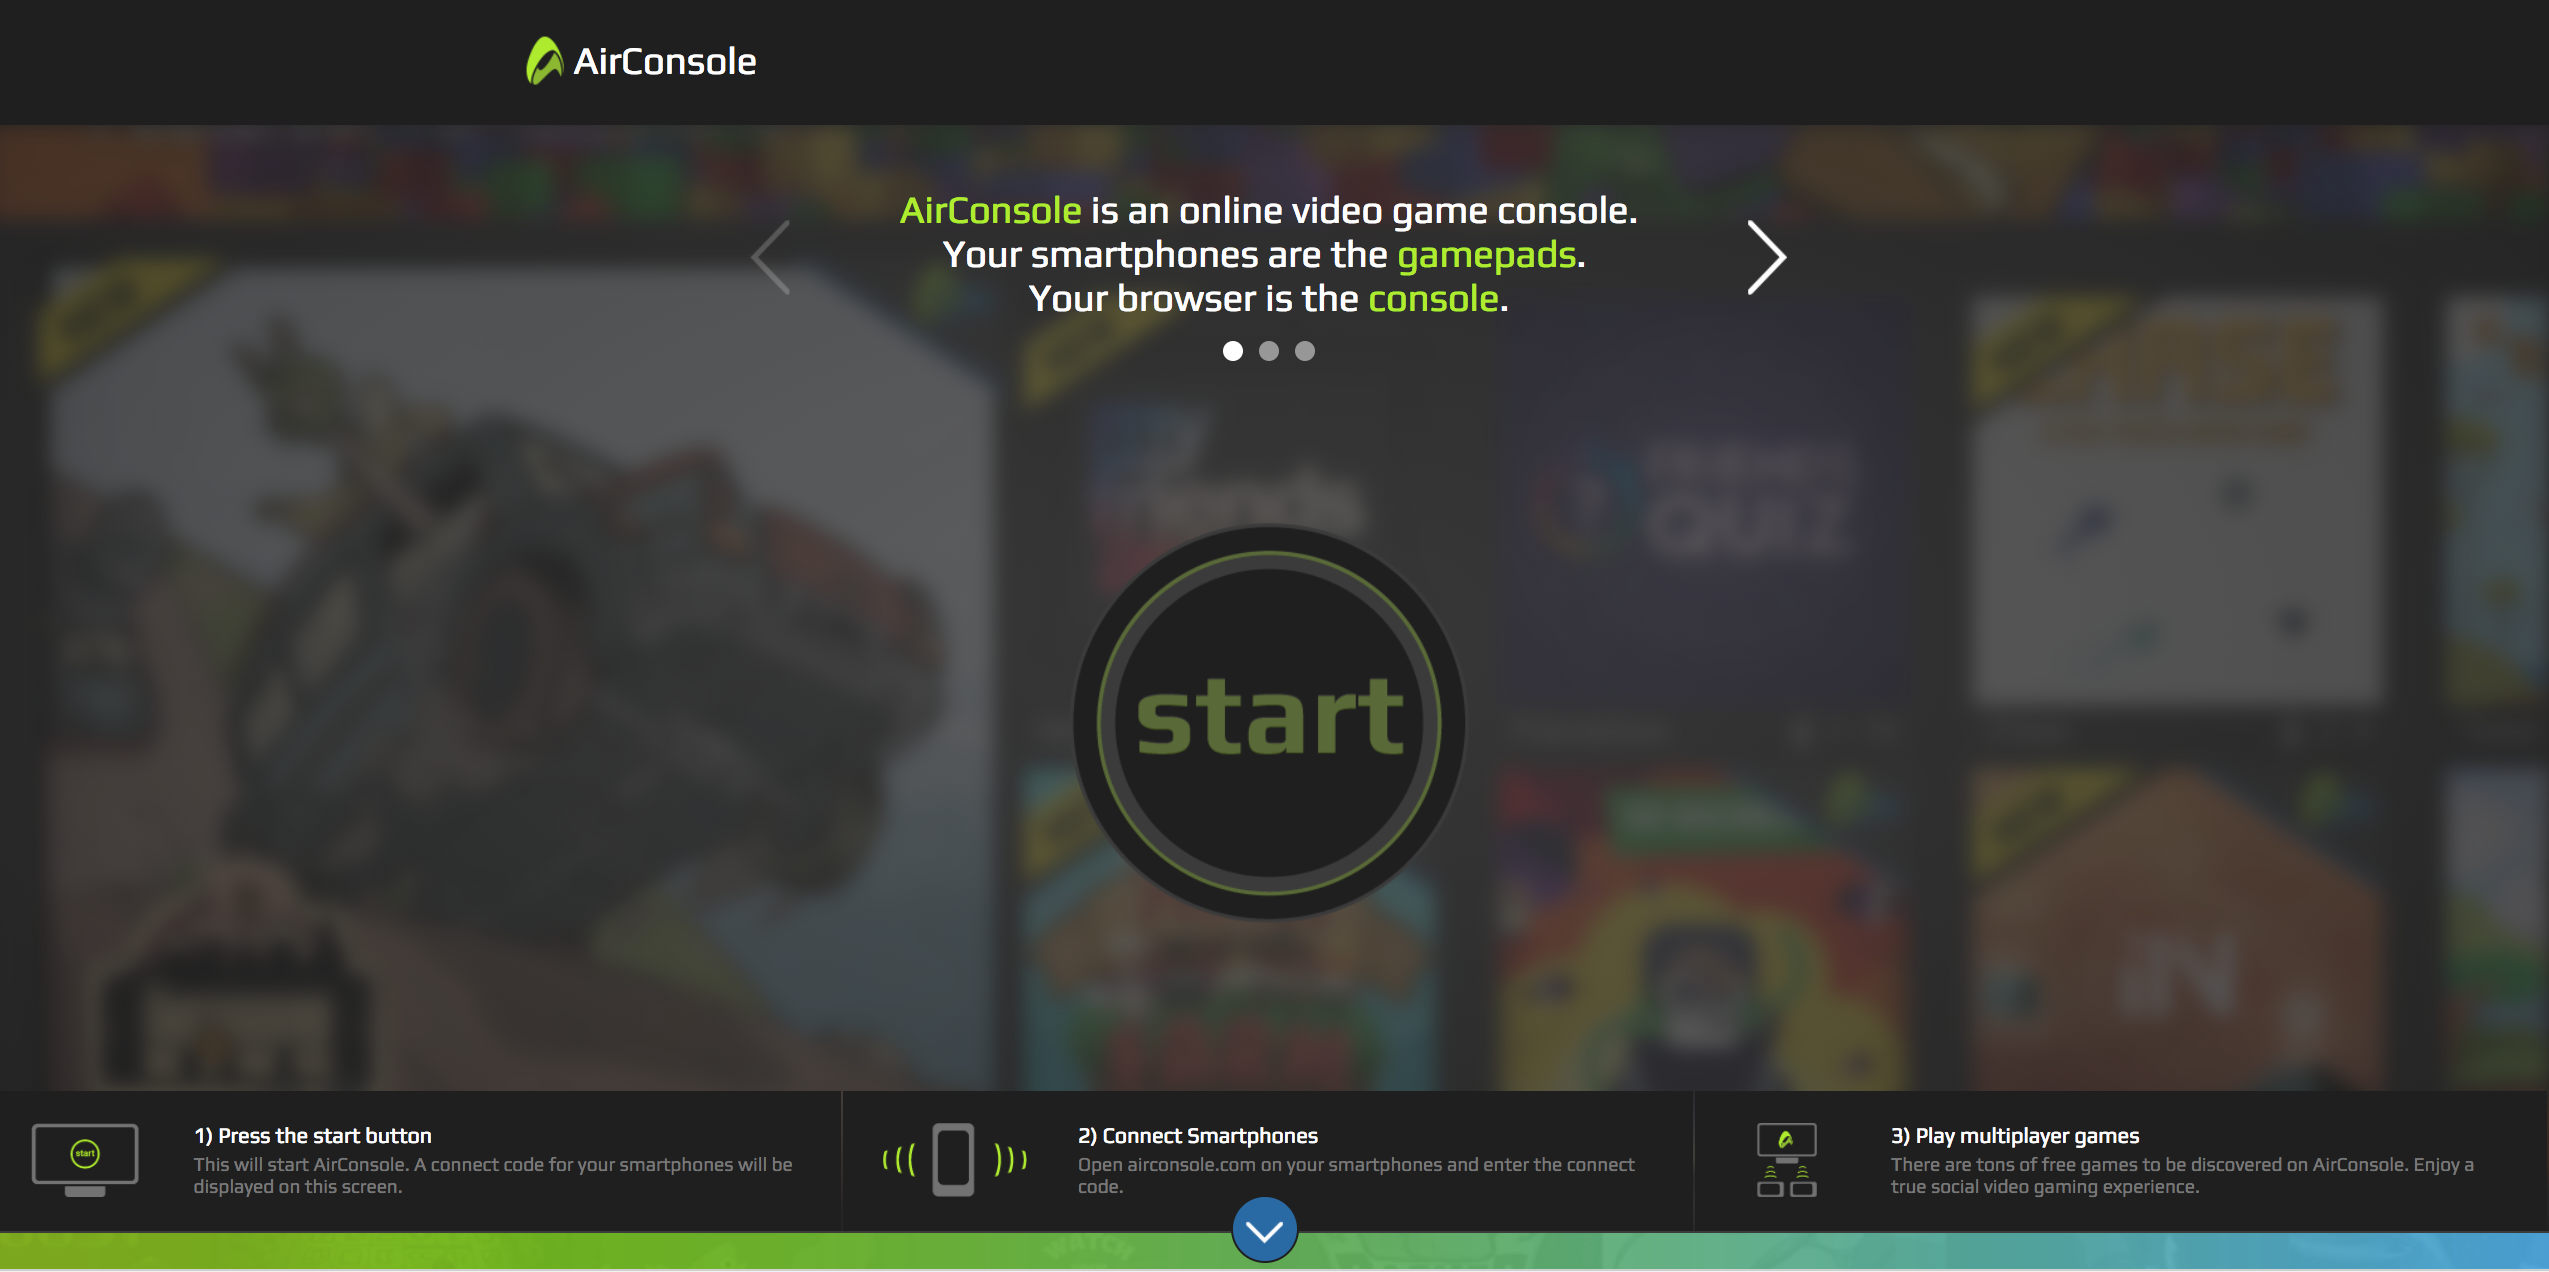
\includegraphics[scale=0.3]{Gambar/con1_home1}
	\caption{Halaman awal web pada \textit{PC browser}.}
	\label{fig:16_con1_home1}
\end{figure}

Setelah tombol \textit{start} ditekan, maka akan muncul halaman berikutnya yang menunjukan kode yang harus dimasukan oleh pemain pada \textit{mobile browser}. 

\begin{figure}[H]
	\centering
	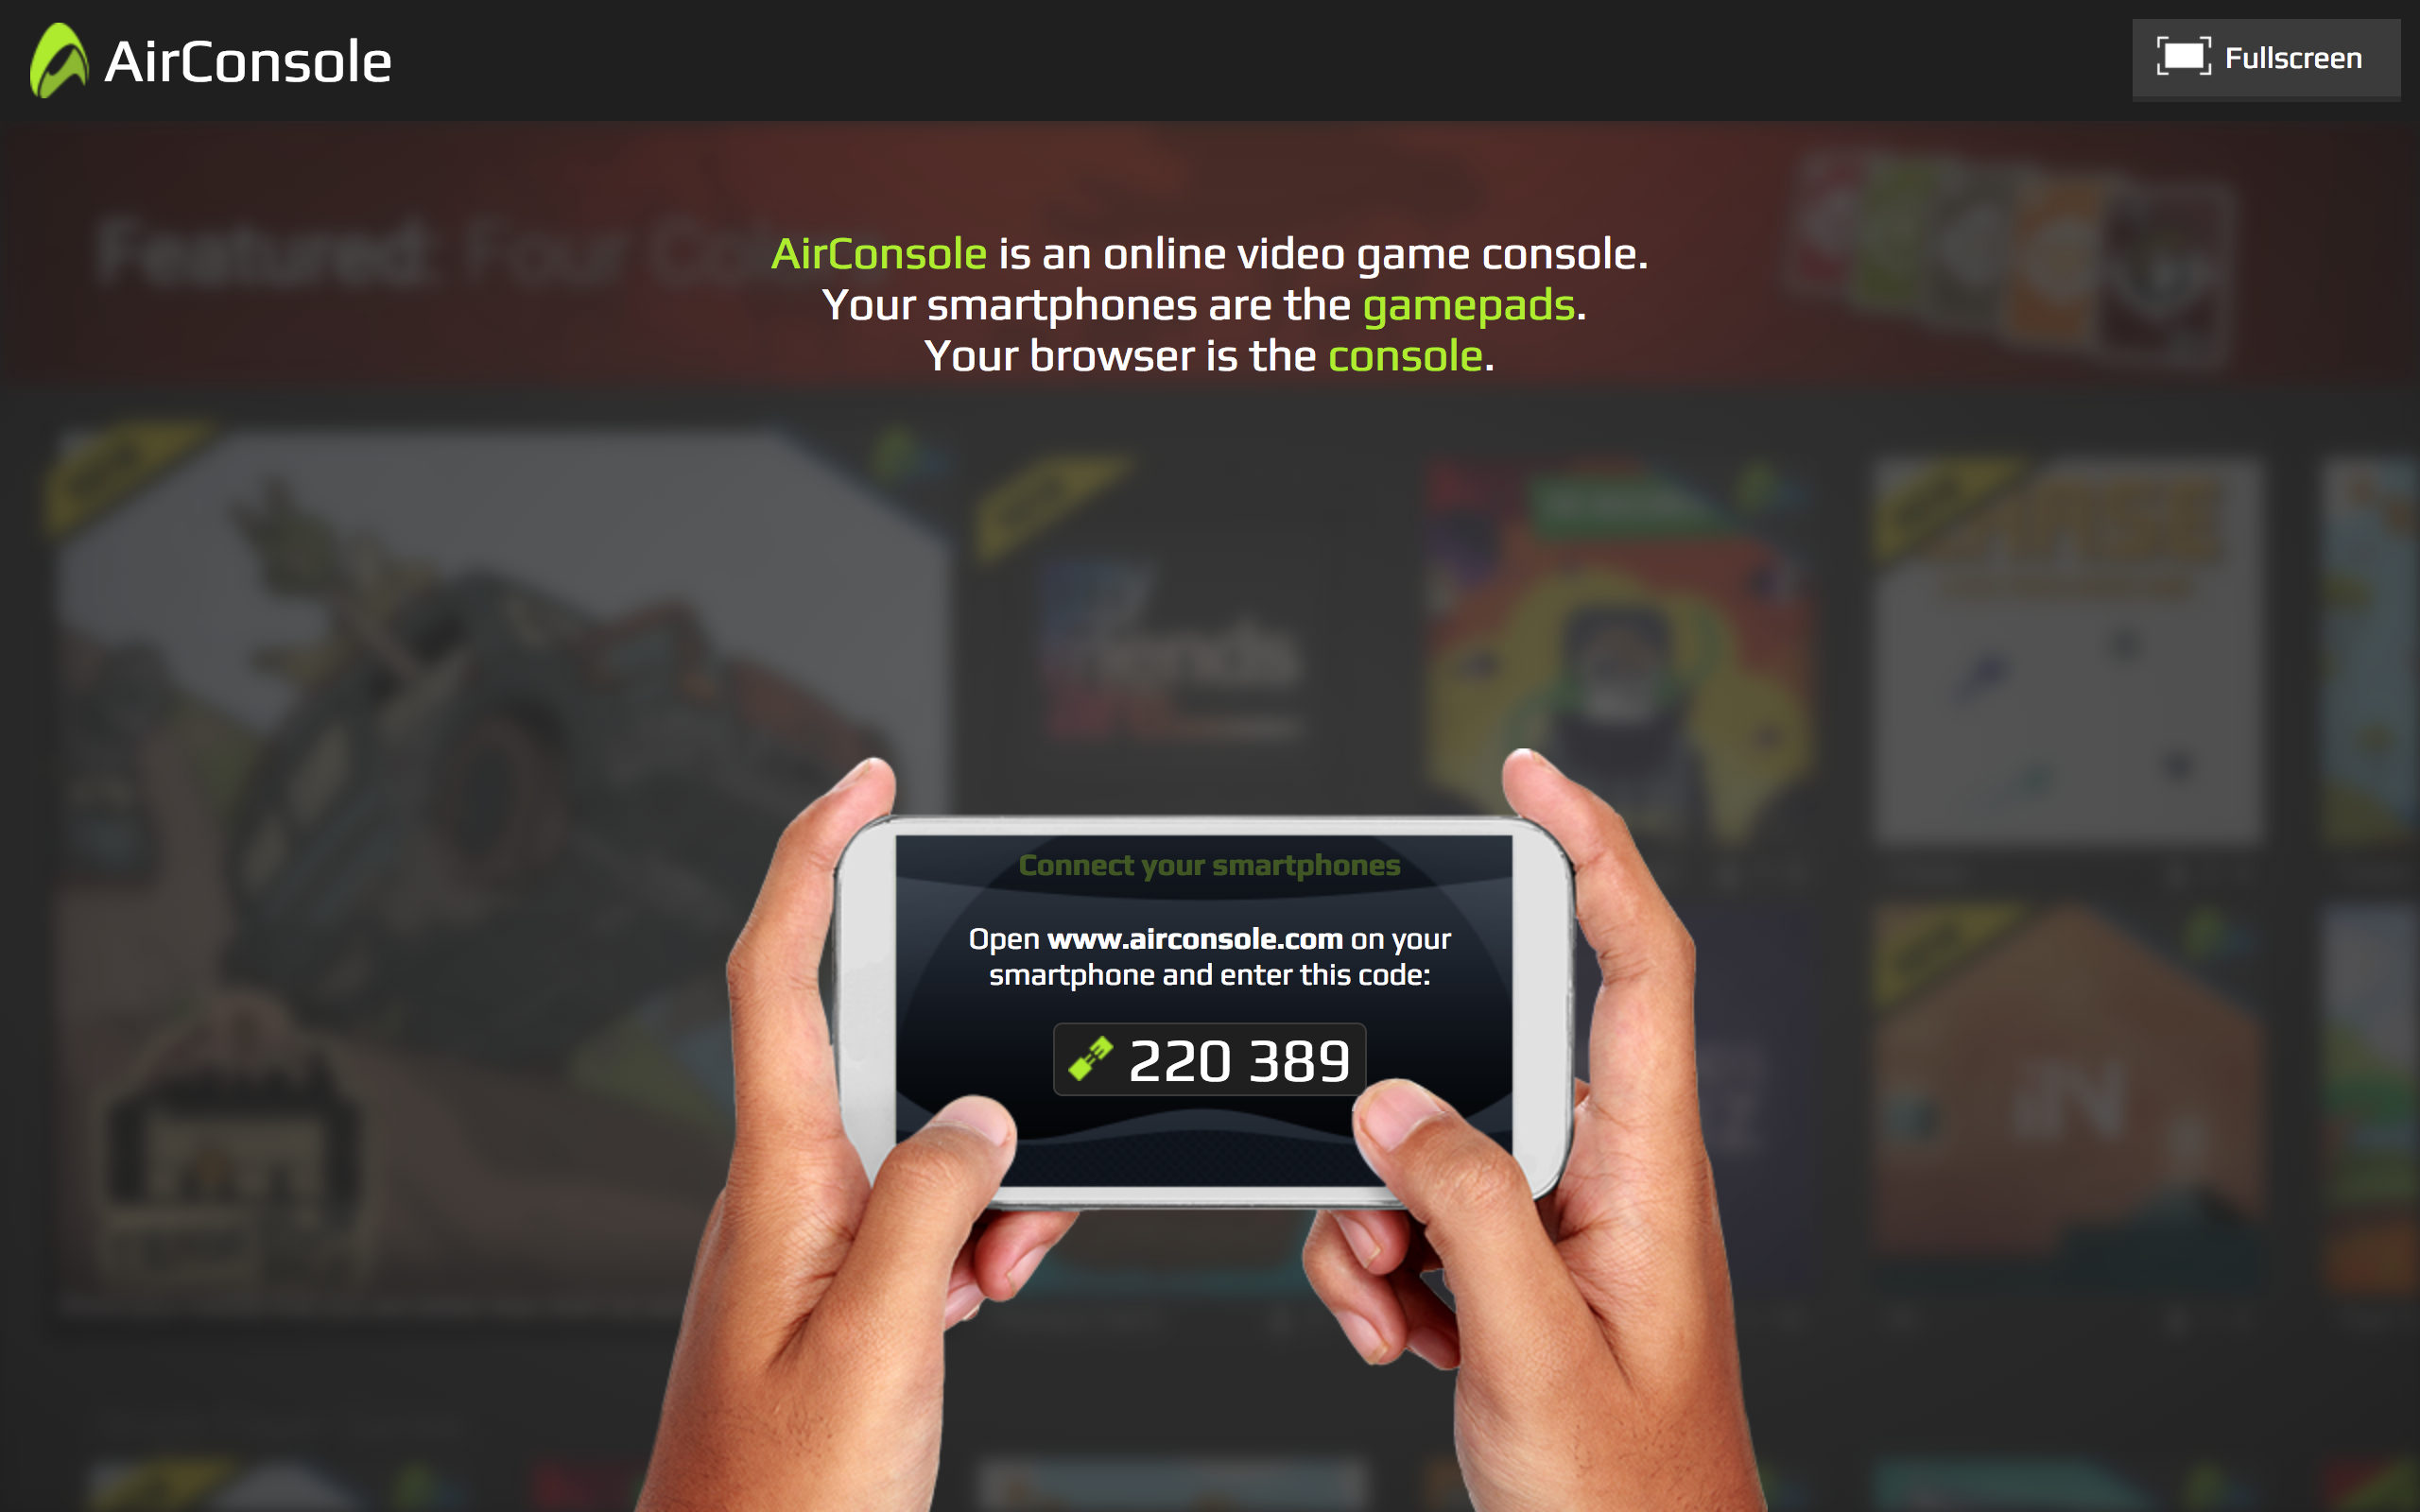
\includegraphics[scale=0.3]{Gambar/con2_code1}
	\caption{Kode yang harus dimasukan oleh pemain pada \textit{mobile browser}.}
	\label{fig:17_con2_code1}
\end{figure}

Pemain harus mengakses alamat web yang sama pada \textit{mobile browser}. Pada halaman awal, pemain akan diminta untuk memilih apakah akan bermain dengan menggunakan aplikasi, atau bermain dengan menggunakan \textit{browser}. 

\begin{figure}[H]
	\centering
	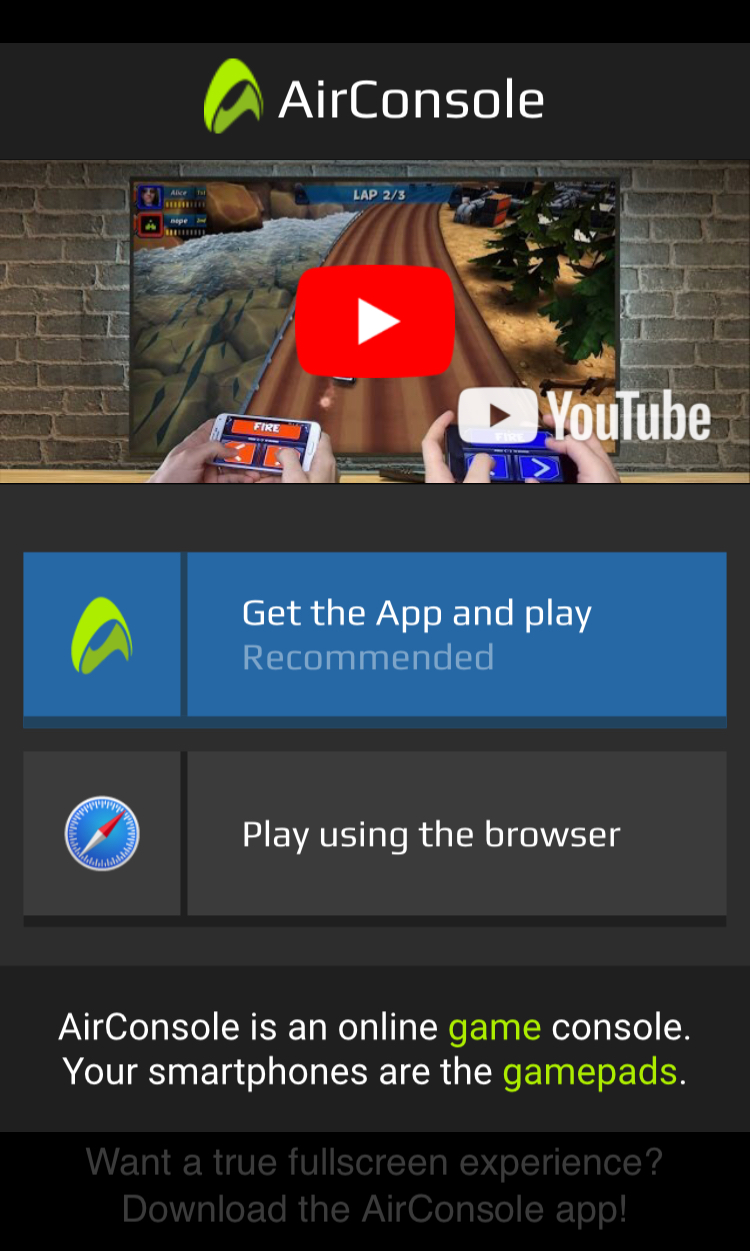
\includegraphics[scale=0.3]{Gambar/air1_home}
	\caption{Halaman awal pada \textit{mobile browser}.}
	\label{fig:18_air1_home}
\end{figure}

\vspace{-3cm}

Dalam analisis ini, penulis memilih untuk bermain menggunakan \textit{browser}. Setelah itu, pemain diminta untuk menekan tombol \textit{'i got the connect code'} untuk memasukan kode yang sudah didapatkan pada \textit{PC browser}.

\begin{figure}[H]
	\centering
	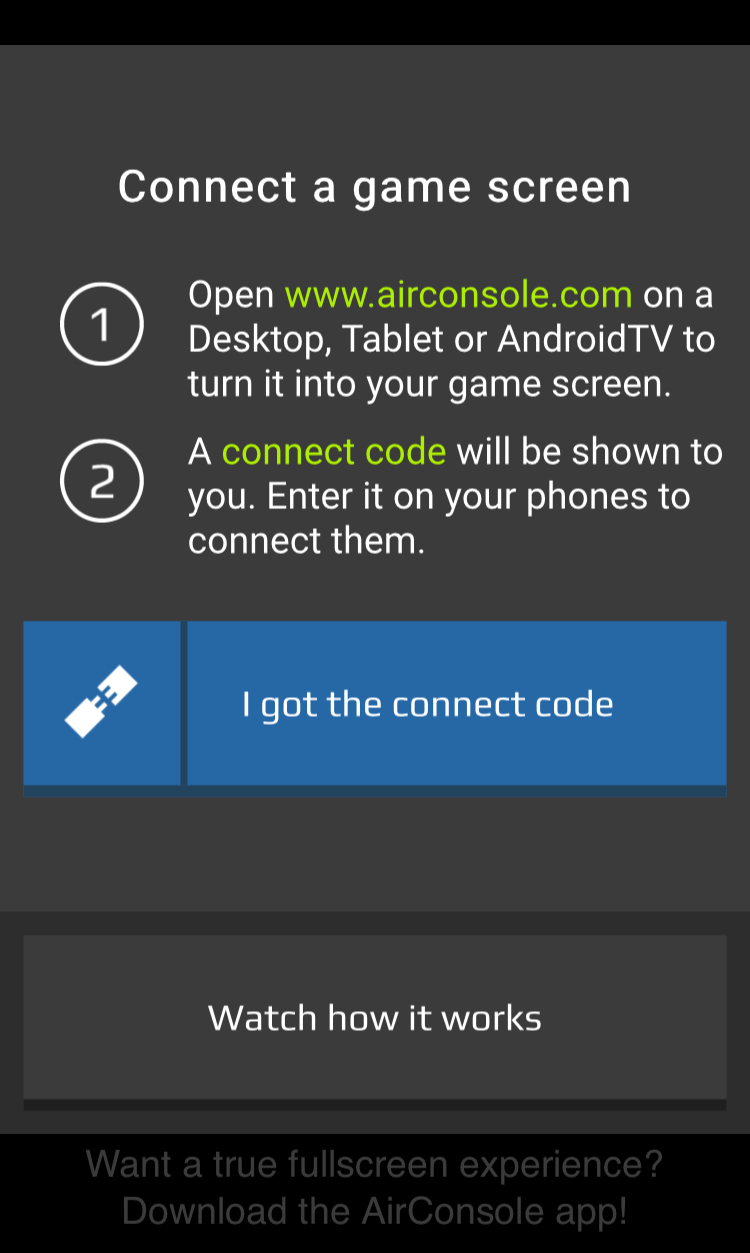
\includegraphics[scale=0.3]{Gambar/air2_code1}
	\caption{Pemain diminta untuk memasukan kode yang sudah didapatkan pada \textit{PC browser}.}
	\label{fig:19_air2_code1}
\end{figure}


Setelah menekan tombol tersebut, pemain dapat mulai memasukan kode yang sudah didapatkan. Kode ini bertujuan untuk proses otentikasi, sehingga para pemain yang dapat bermain dalam satu sesi yang sama, hanya para pemain yang mengetahui kode tersebut.

\begin{figure}[H]
	
	\centering
	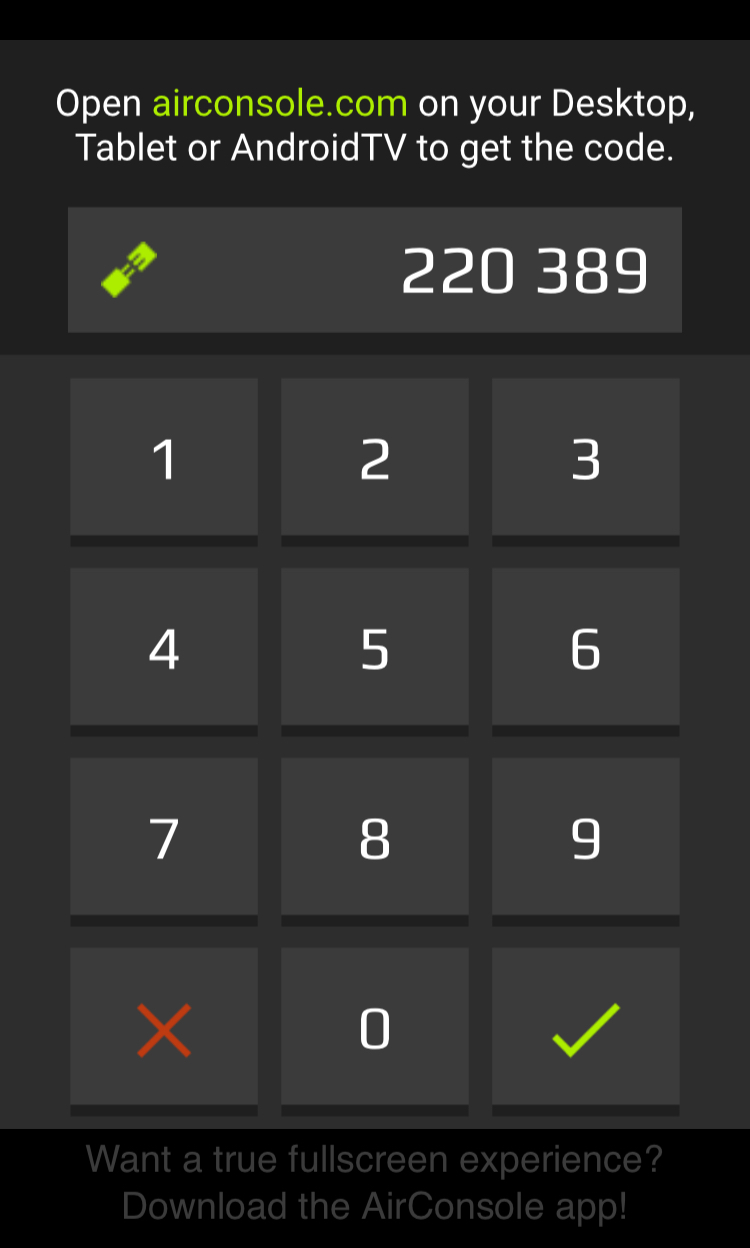
\includegraphics[scale=0.3]{Gambar/air3_code2}
	\caption{Pemain diminta untuk memasukan kode yang sudah didapatkan pada \textit{PC browser}.}
	\label{fig:20_air3_code2}
	
	
\end{figure}


Setelah pemain memasukan kode, maka halaman web di \textit{PC} dan \textit{smartphone} akan berubah. Pada \textit{PC}, halaman akan menunjukan berbagai jenis permainan yang dapat dipilih. Pada \textit{smartphone}, halaman akan berubah menjadi pengendali permainan, dimana pemain dapat menggerakan halaman yang ada di \textit{PC} dengan menggunakan \textit{smartphone}.

\begin{figure}[H]
	\centering
	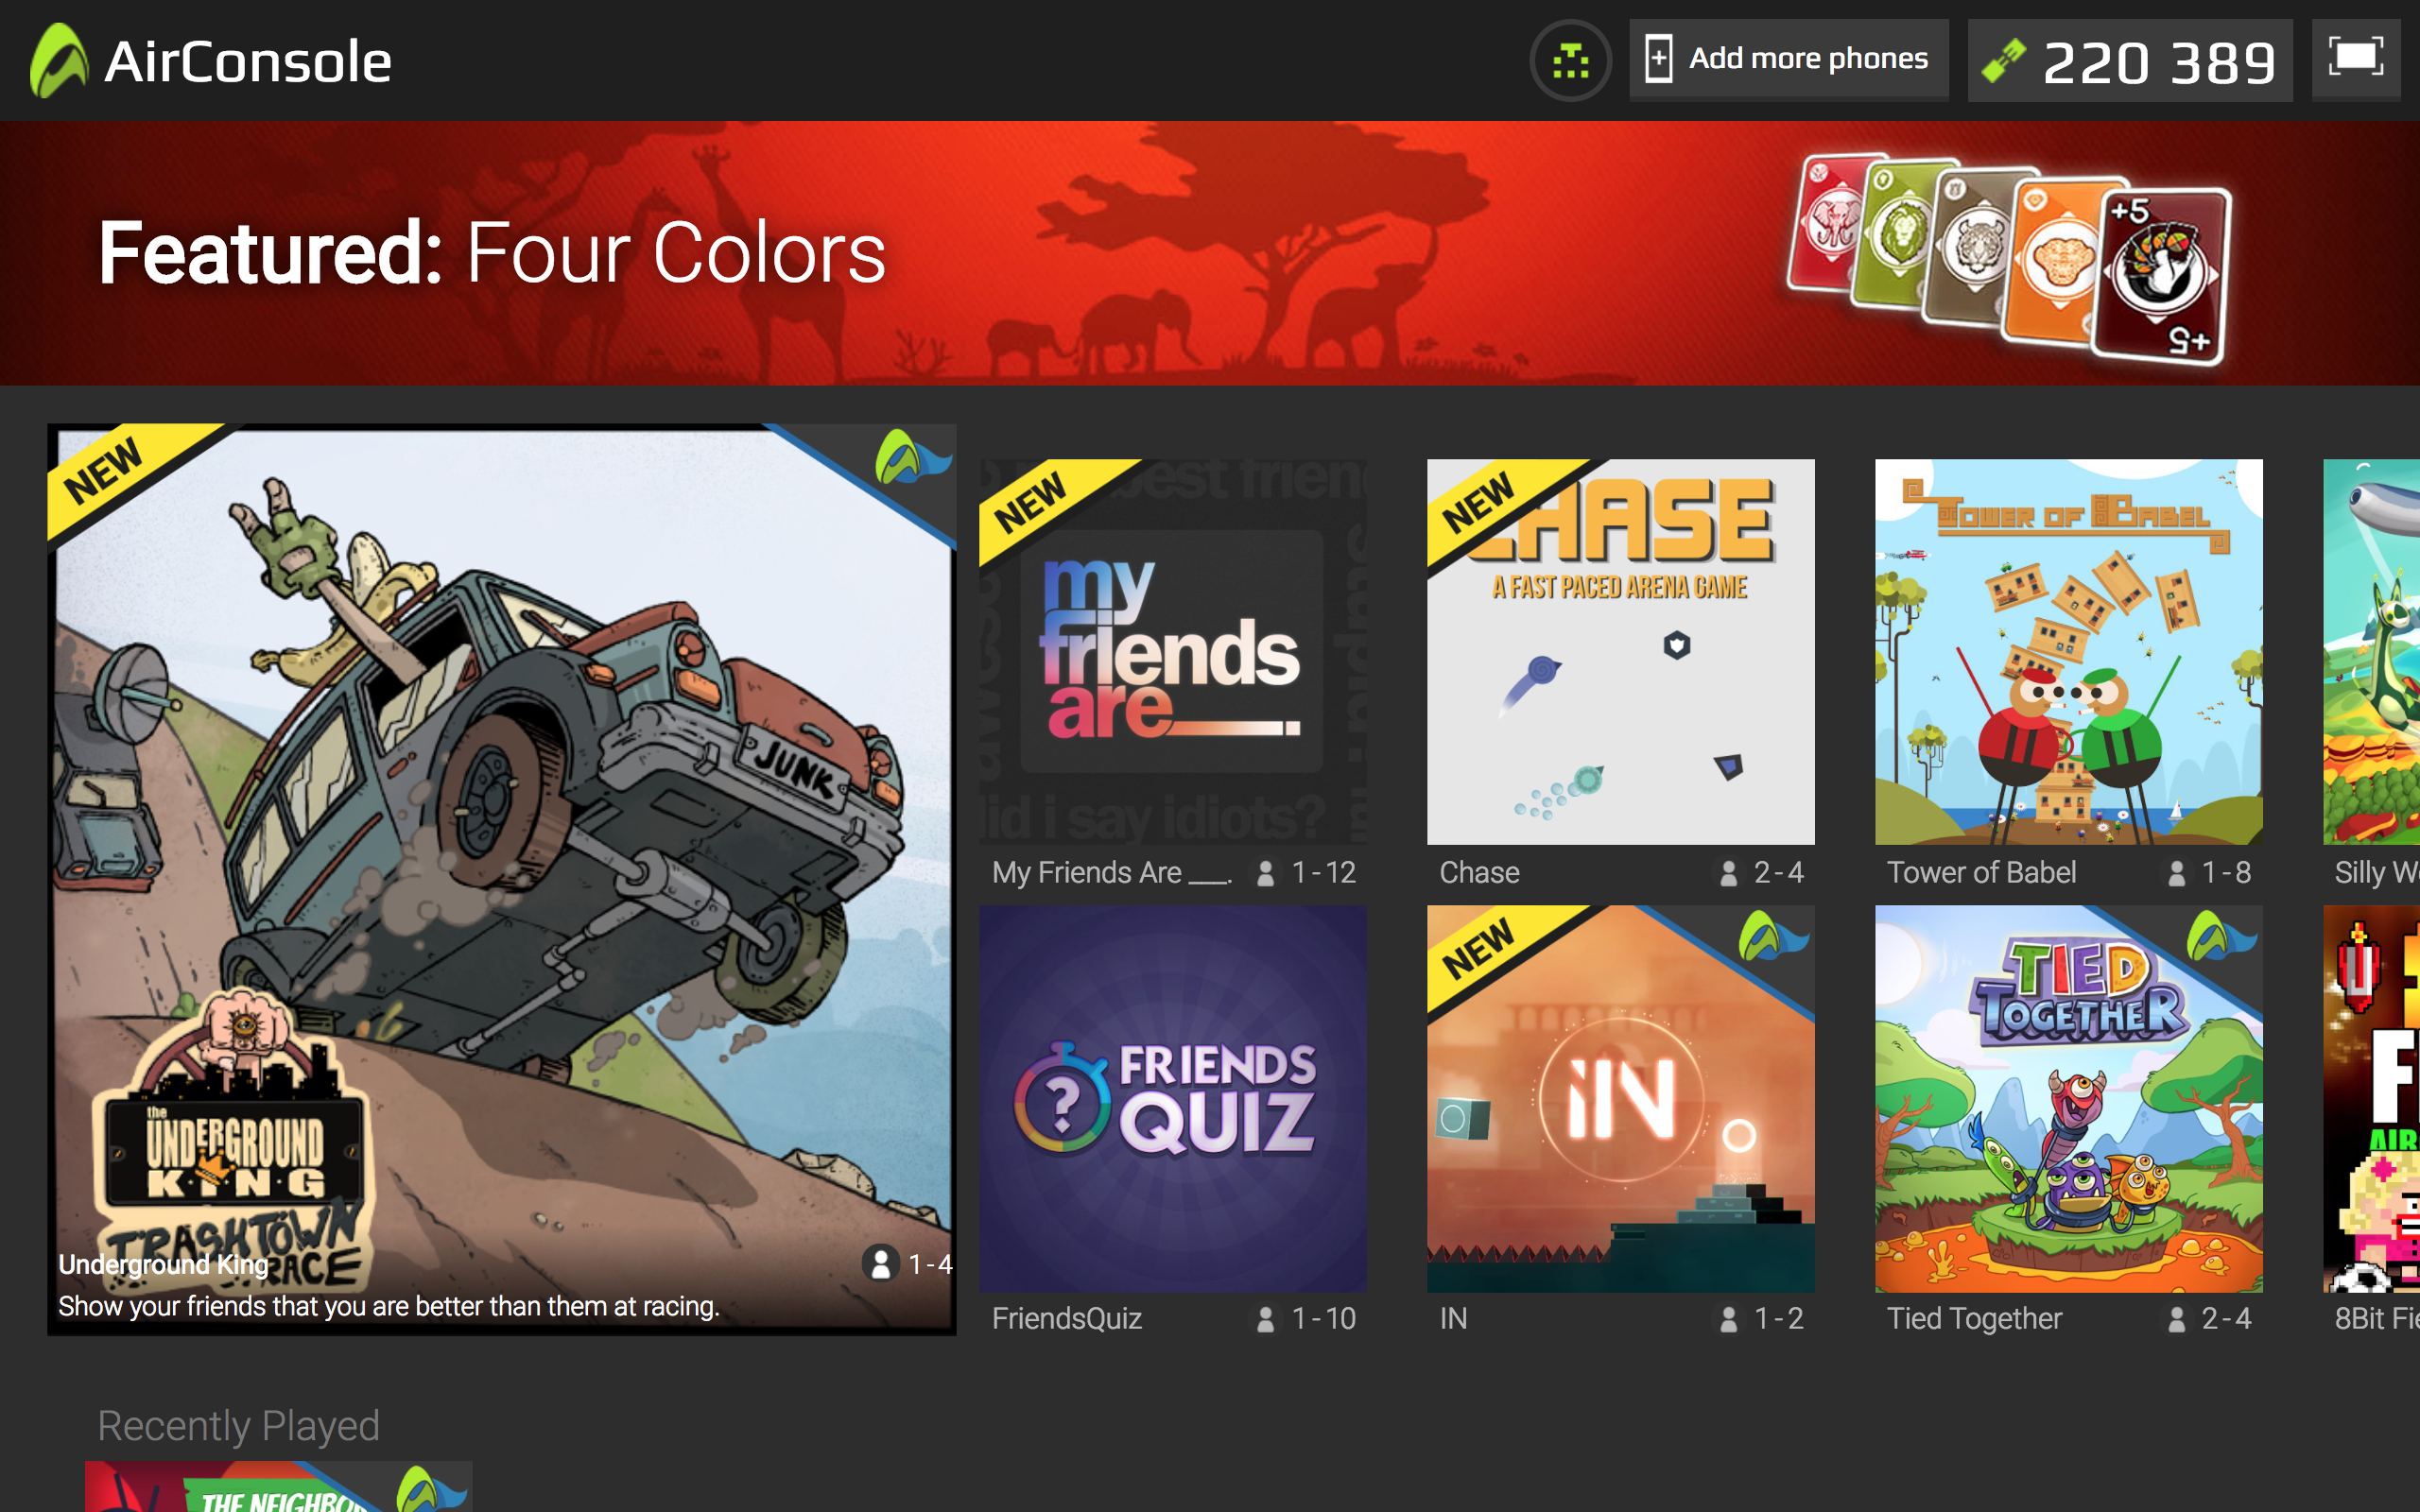
\includegraphics[scale=0.3]{Gambar/con3_play1}
	\caption{Halaman pada \textit{PC} yang menunjukan berbagai permainan yang dapat dipilih.}
	\label{fig:21_con3_play1}
\end{figure}

\begin{figure}[H]
	\centering
	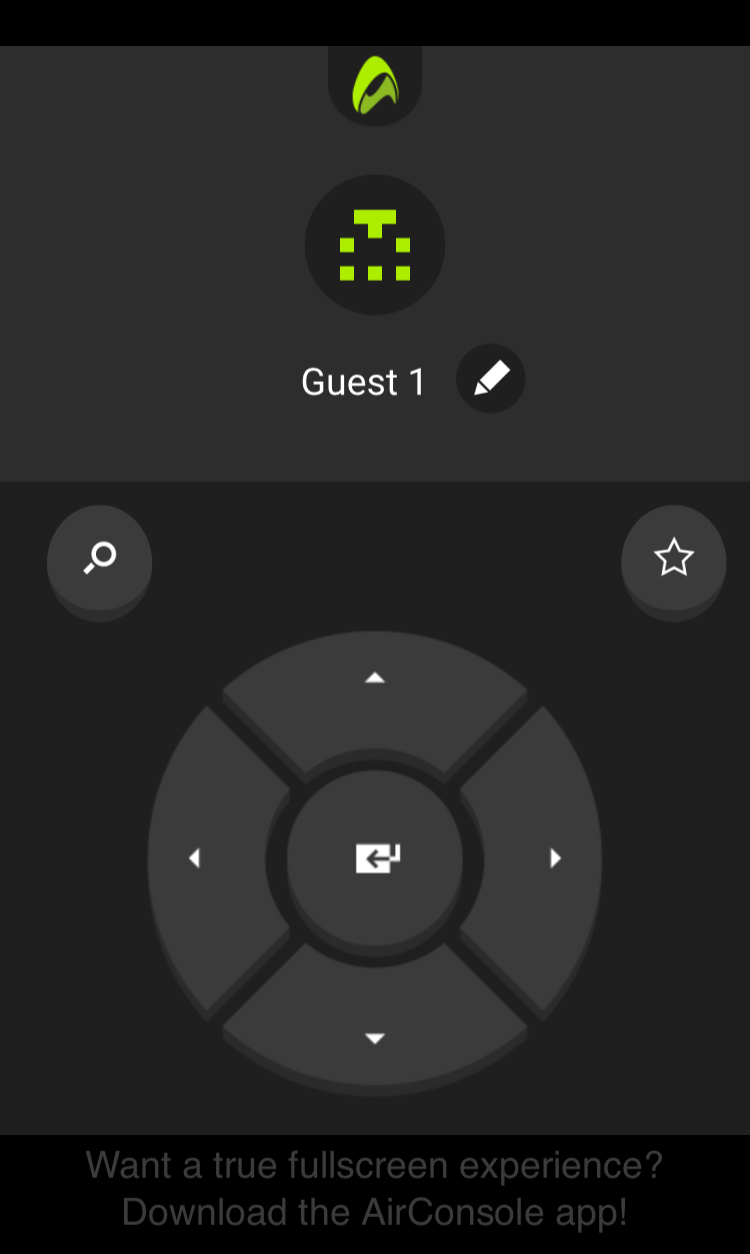
\includegraphics[scale=0.3]{Gambar/air4_play1}
	\caption{Halaman pada \textit{smartphone} yang berfungsi sebagai pengendali.}
	\label{fig:22_air4_play1}
\end{figure}

Dalam analisis ini, penulis memilih untuk memainkan permainan yang bernama The Neighborhood. Permainan ini sejenis permainan Angry Birds. Permainan ini bercerita tentang dua kelompok yang bertetangga, dimana kelompok tersebut bermusuhan dan berusaha untuk saling menghancurkan satu sama lain. Tujuan dari permainan ini yaitu lebih dulu menghancurkan anggota kelompok tetangga. Setelah memilih permainan tersebut, halaman pada \textit{PC} dan \textit{smartphone} akan berubah. Pada \textit{smartphone}, pemain akan diminta untuk merubah mode tampilan \textit{smartphone} menjadi \textit{landscape}.

\begin{figure}[H]
	\centering
	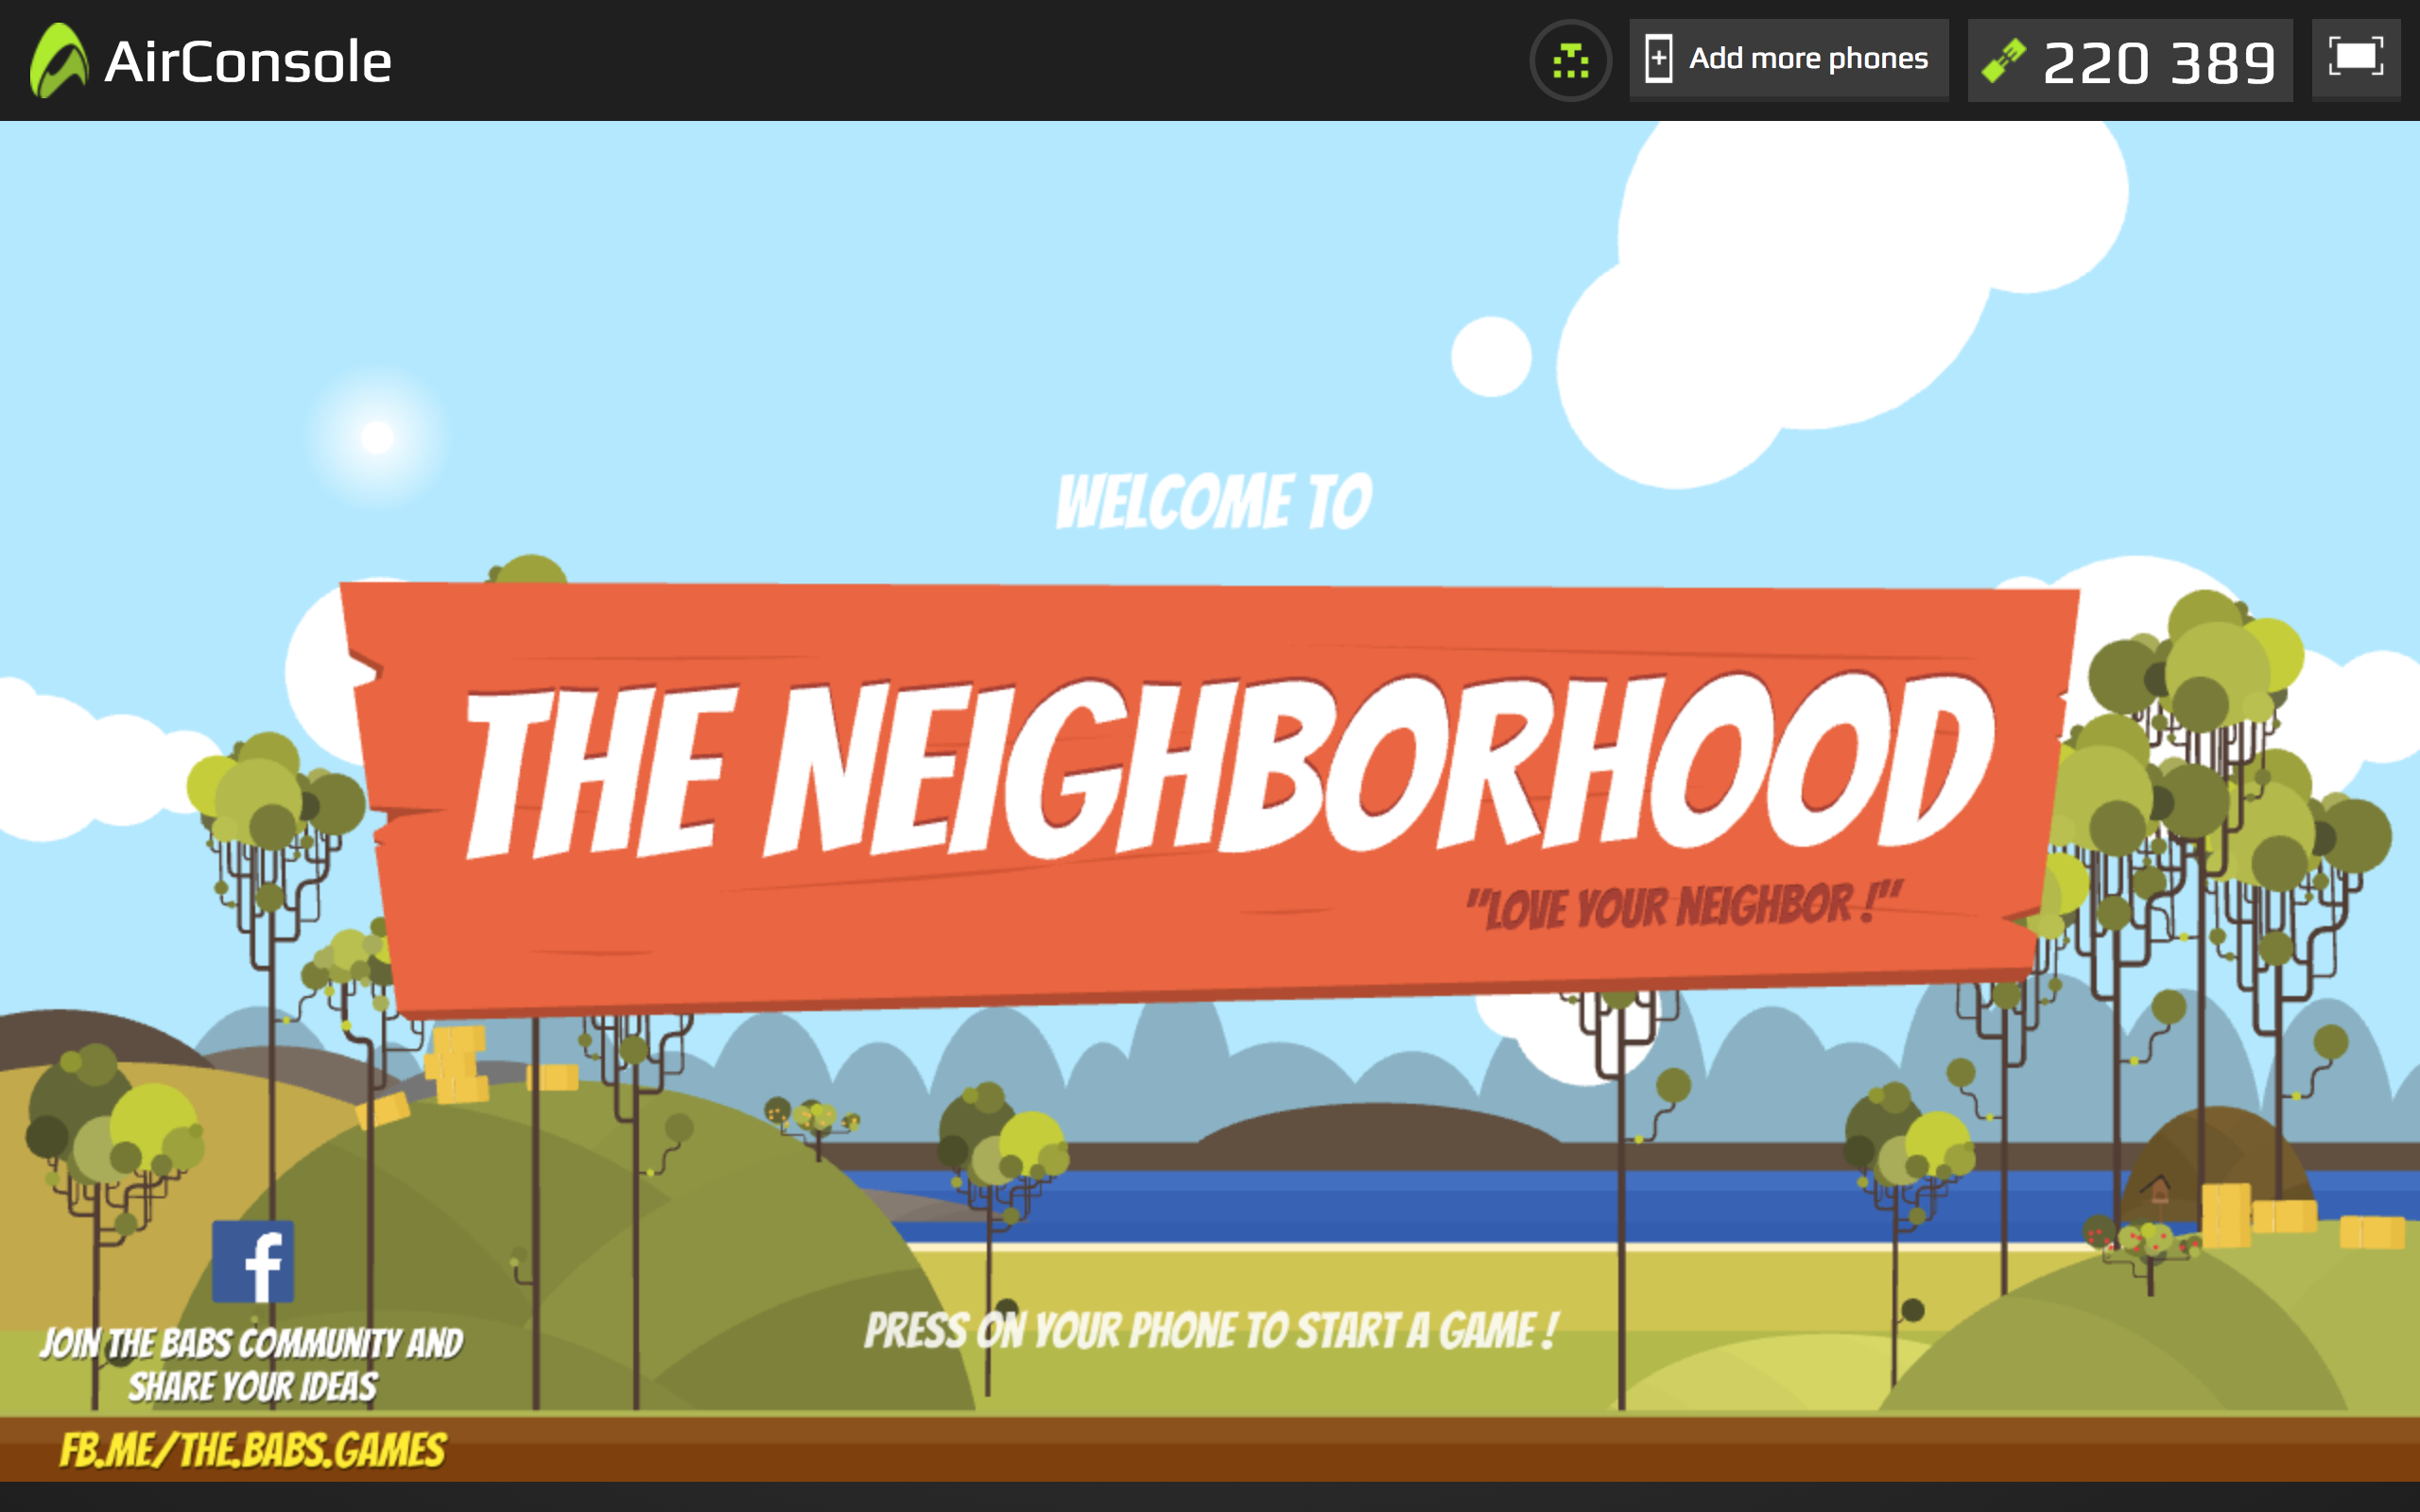
\includegraphics[scale=0.3]{Gambar/con5_play3}
	\caption{Halaman awal permainan The Neighborhood pada \textit{PC}.}
	\label{fig:23_con5_play3}
\end{figure}

\begin{figure}[H]
	\centering
	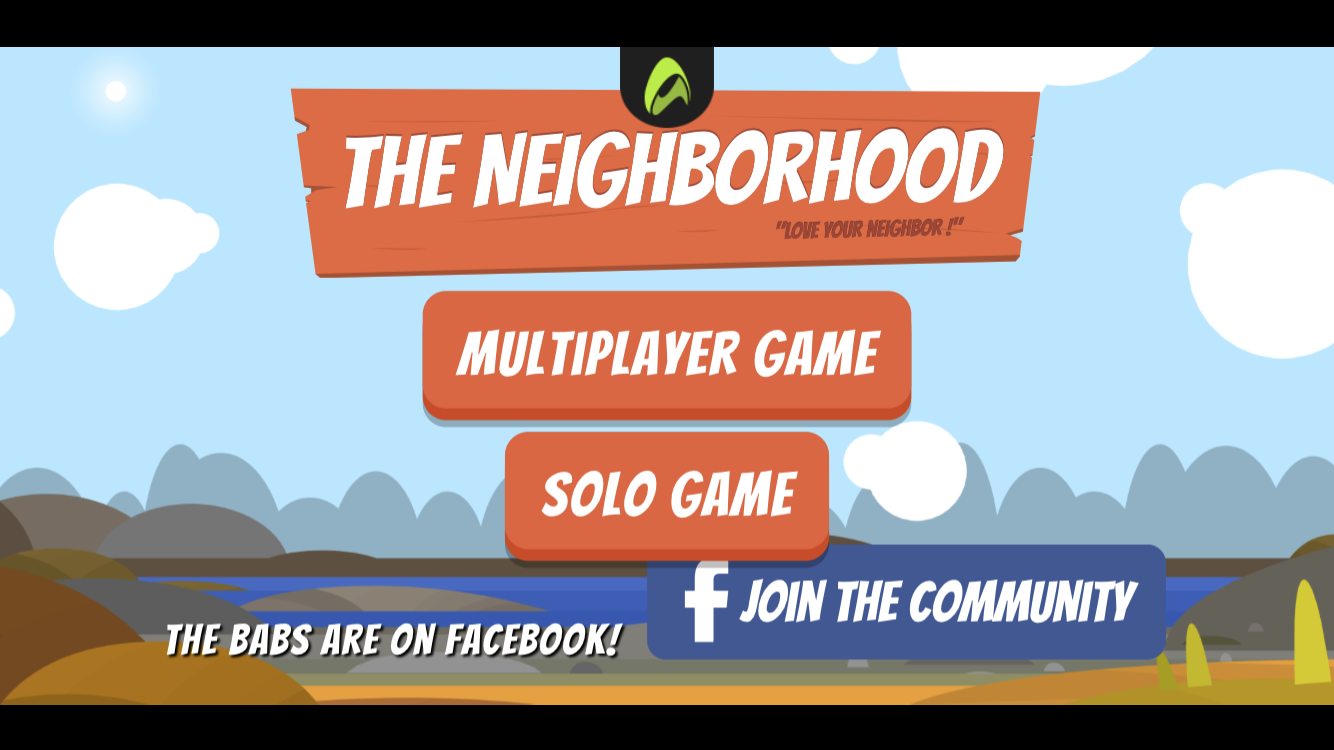
\includegraphics[scale=0.3]{Gambar/air6_play3}
	\caption{Halaman awal permainan The Neighborhood pada \textit{smartphone}.}
	\label{fig:24_air6_play3}
\end{figure}

Cara bermain dari permainan tersebut yaitu dengan menggunakan \textit{smartphone}, dimana pemain harus menekan layar \textit{smartphone}, kemudian menariknya sesuai dengan arah yang berlawanan dengan lawan, lalu melepas jari dari layar \textit{smartphone} dengan tujuan untuk melempar suatu benda dari ketapel. Semakin jauh pemain menarik, maka lontaran benda tersebut akan semakin kencang mengenai lawan.

\begin{figure}[H]
	\centering
	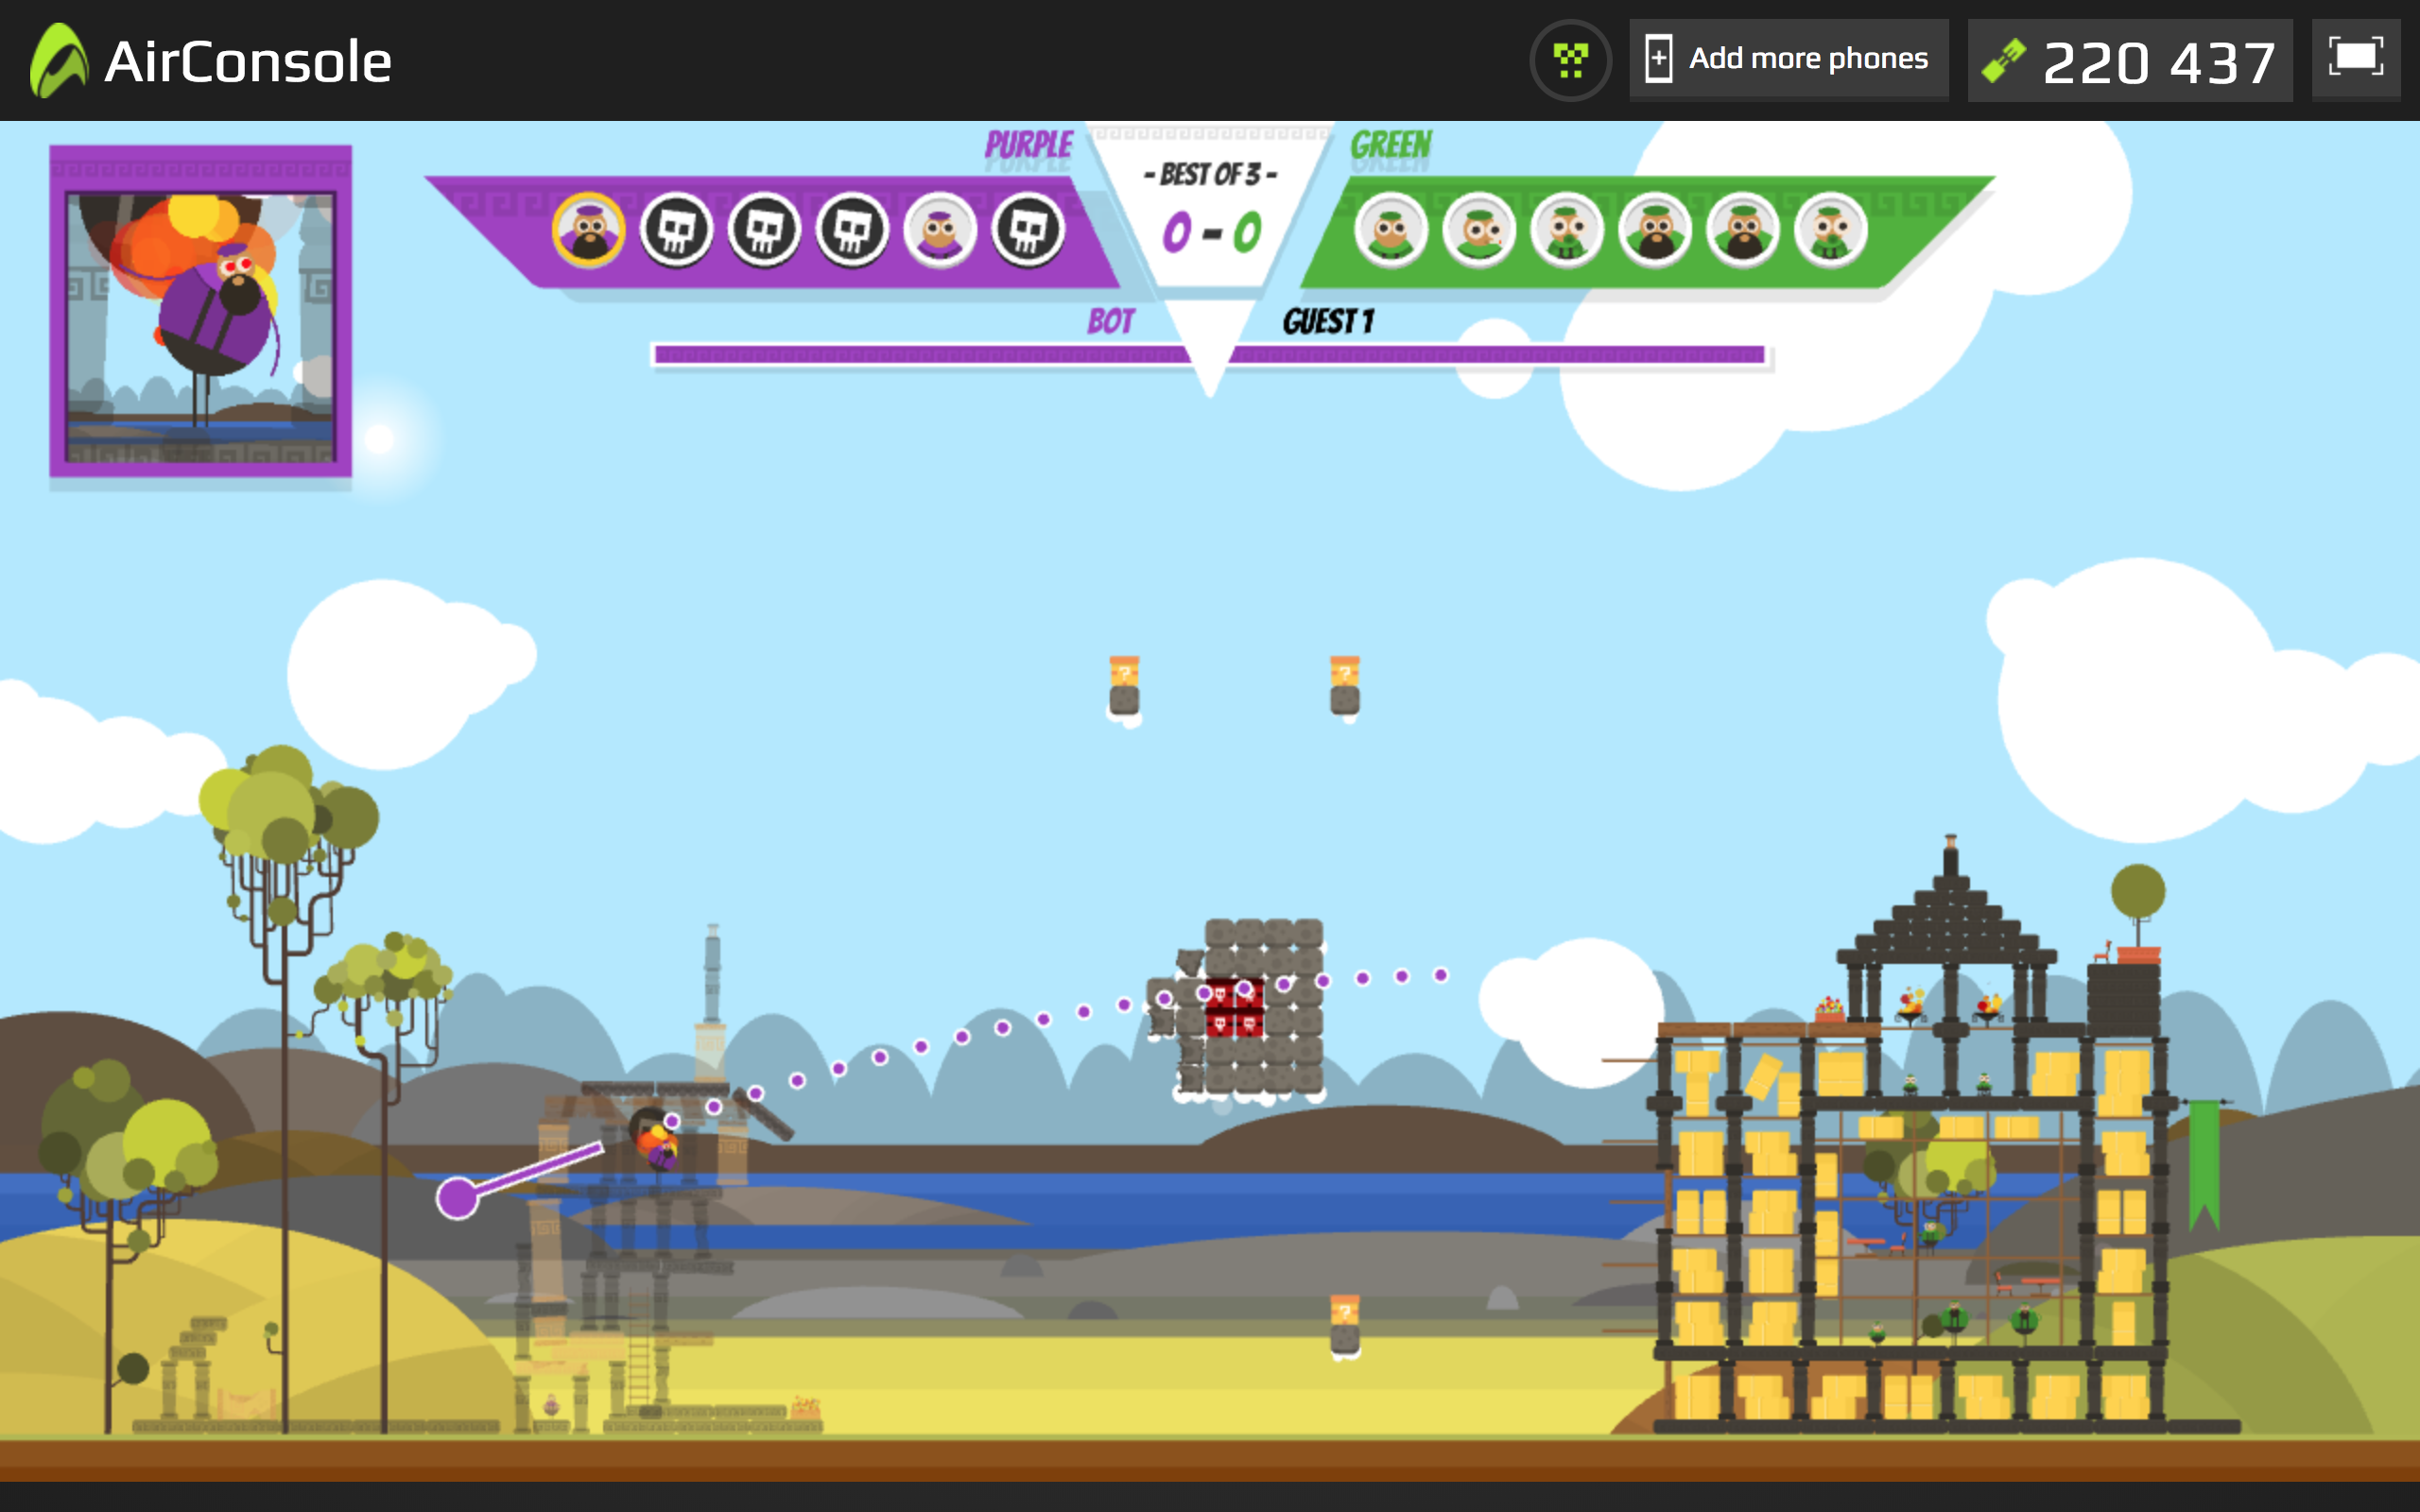
\includegraphics[scale=0.3]{Gambar/con7_play5}
	\caption{Halaman pada \textit{PC} dimana permainan sedang berlangsung.}
	\label{fig:25_con7_play5}
\end{figure}

\begin{figure}[H]
	\centering
	
\includegraphics[scale=0.3]{Gambar/air7_play4}
	\caption{Halaman pada \textit{smartphone} dimana permainan sedang berlangsung.}
	\label{fig:26_air7_play4}
\end{figure}

Apabila memenangkan permainan tersebut, maka pemain dapat memilih untuk keluar dari permainan atau melanjutkan permainannya kembali.

\begin{figure}[H]
	\centering
	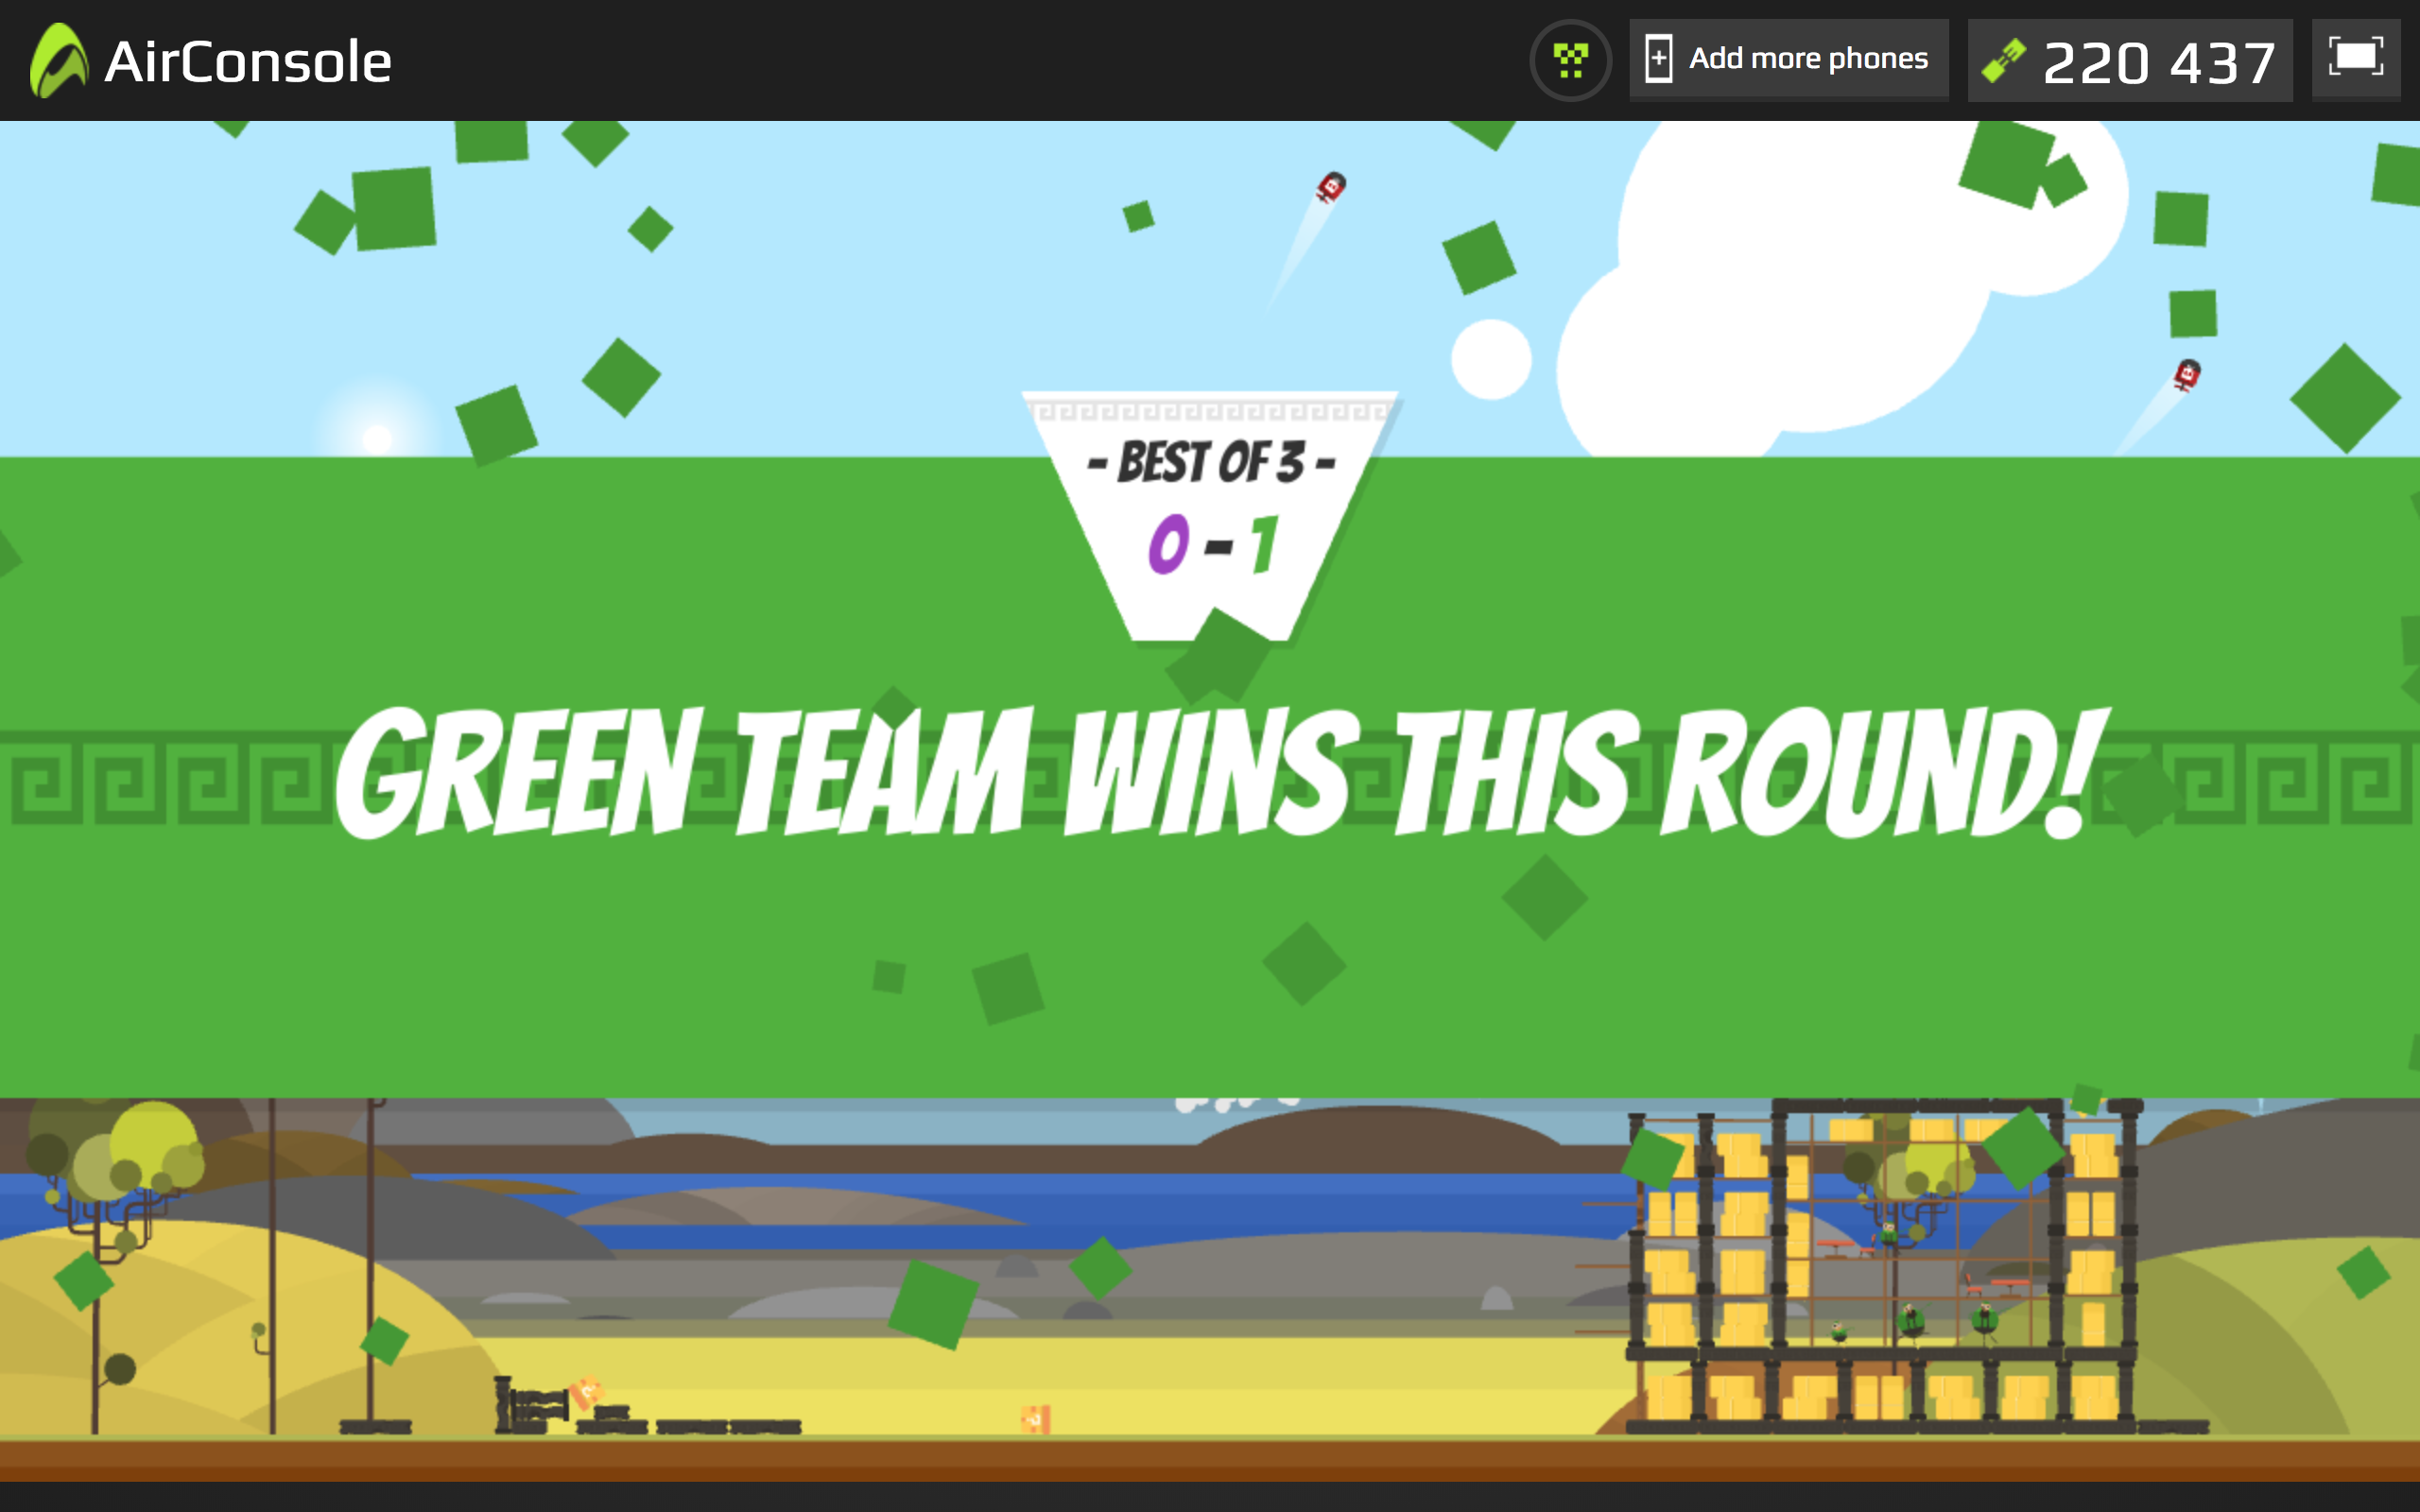
\includegraphics[scale=0.3]{Gambar/con8_play6}
	\caption{Halaman pada \textit{PC} apabila permainan sudah dimenangkan.}
	\label{fig:27_con8_play6}
\end{figure}

\begin{figure}[H]
	\centering
	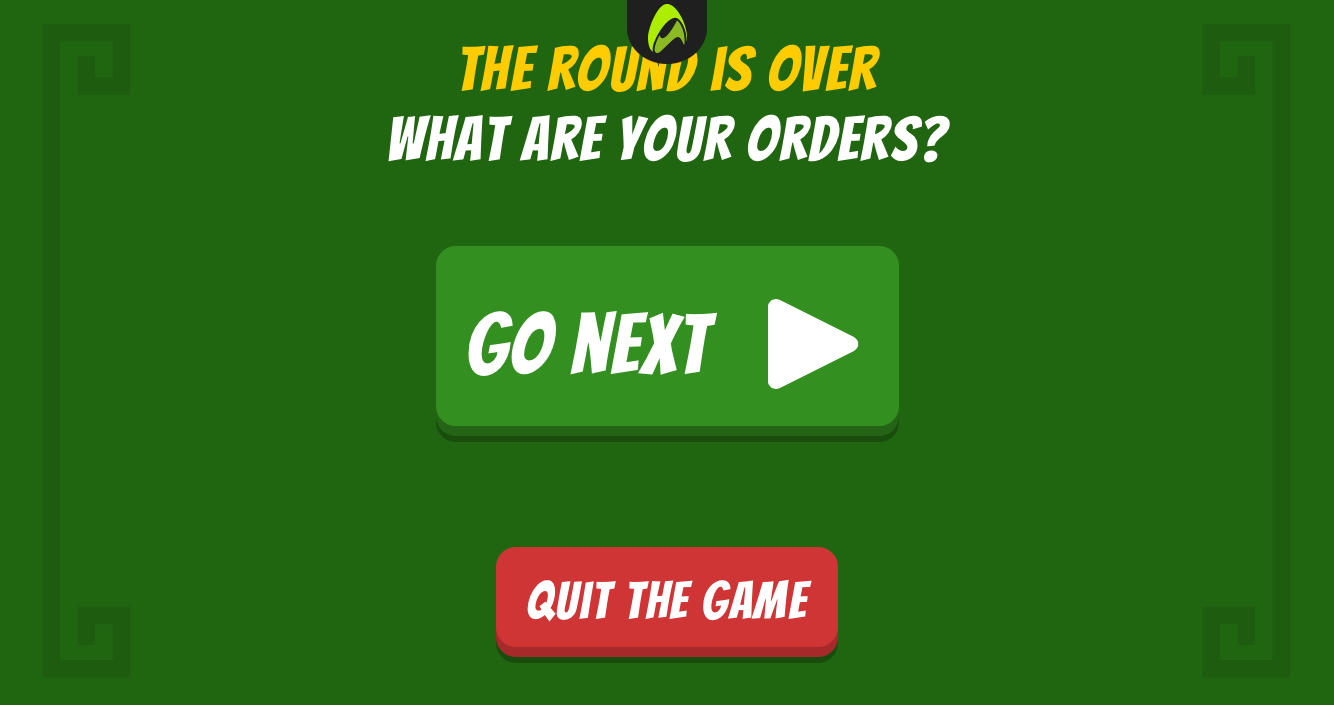
\includegraphics[scale=0.3]{Gambar/air8_finish}
	\caption{Halaman pada \textit{smartphone} apabila permainan sudah dimenangkan.}
	\label{fig:28_air8_finish}
\end{figure}

Dari ketiga percobaan yang sudah dilakukan, ada beberapa hal yang dapat diperbaiki dari permainan berbasis web tersebut. Percobaan pertama menunjukan hasil yang bagus, dimana koneksi antara \textit{smartphone} dan \textit{PC} tidak putus saat permainan berlangsung, dan juga tidak ada keterlambatan antara gerakan pada \textit{smartphone} dan \textit{PC}. Pada percobaan kedua, apabila \textit{browser} pada \textit{PC} ditutup pada saat permainan berlangsung, maka koneksi akan terputus. Tetapi, tampilan pada \textit{smartphone} tidak menunjukan bahwa adanya koneksi yang terputus, sehingga pemain tidak mengetahui apakah permainan masih dapat berlangsung atau tidak. Tampilan hanya akan langsung kembali pada halaman awal permainan. Begitupun dengan percobaan ketiga, apabila \textit{browser} pada \textit{smartphone} ditutup pada saat permainan sedang berlangsung, maka koneksi akan terputus. Tampilan pada \textit{PC} hanya menunjukan tanda kecil bahwa telah terjadi pemutusan koneksi pada \textit{smartphone}, yaitu tanda x pada bagian atas tampilan yang ditunjukan seperti gambar berikut:

\begin{figure}[H]
	\centering
	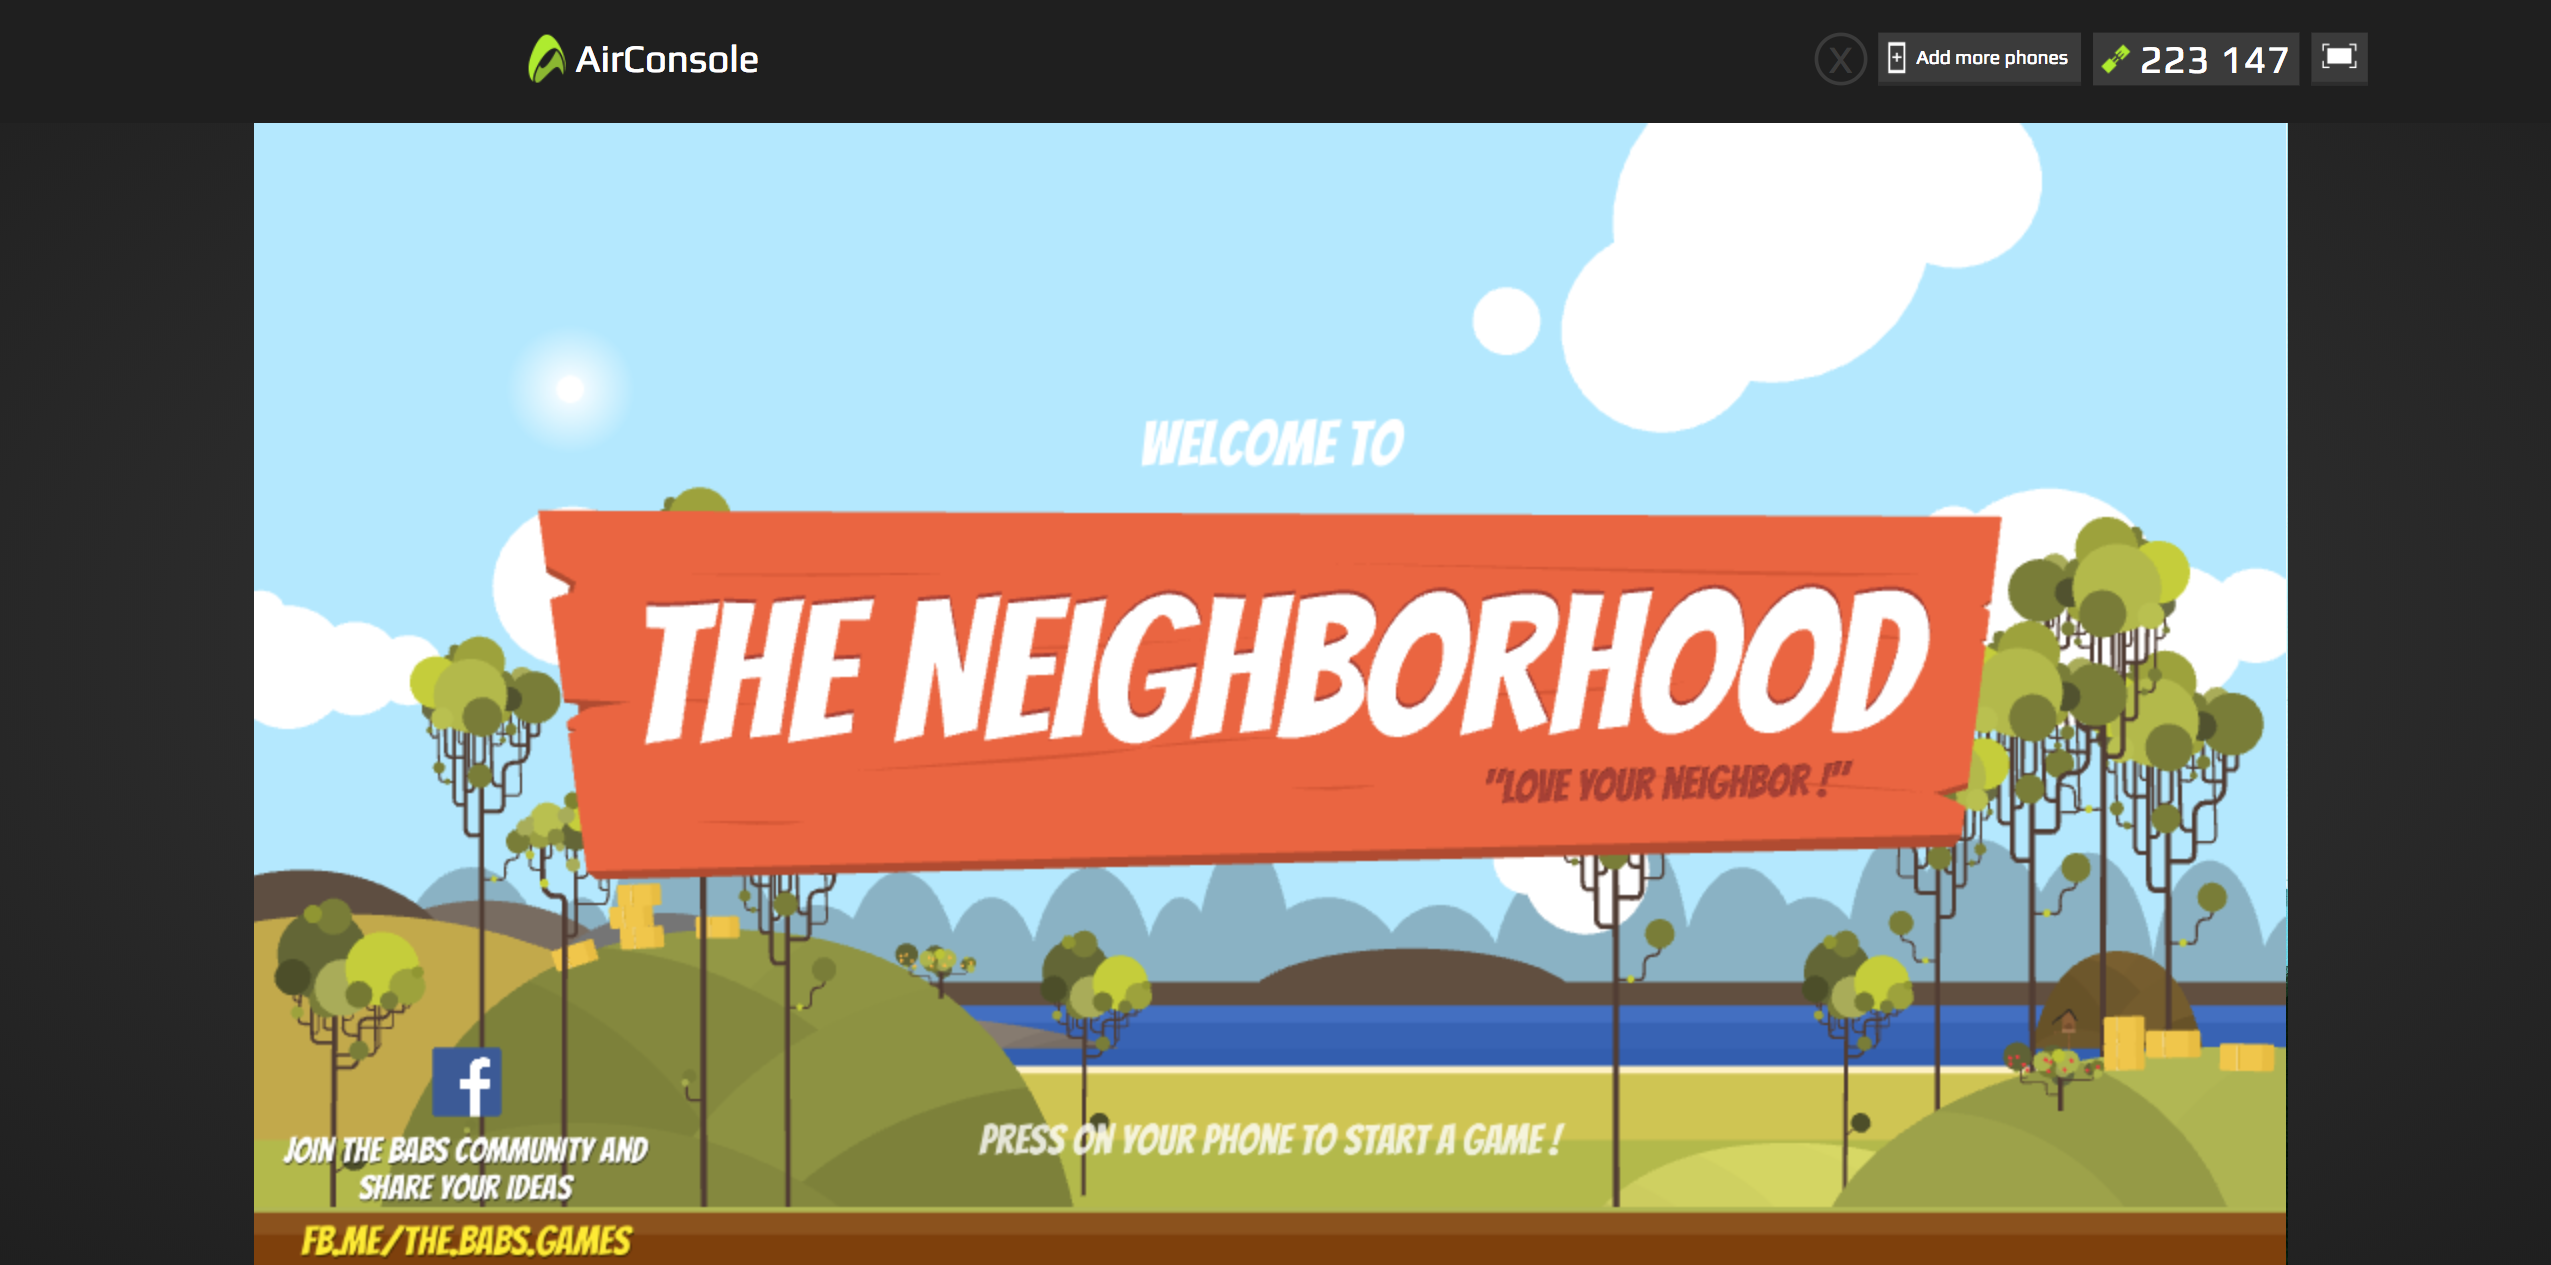
\includegraphics[scale=0.3]{Gambar/con9_play7}
	\caption{Halaman pada \textit{PC} yang menunjukan pemutusan koneksi.}
	\label{fig:29_con9_play7}
\end{figure}

Perbaikan yang dapat dilakukan adalah dengan memberi \textit{feedback} yang lebih jelas pada pemain, apabila ada kesalahan pada aplikasi yang terjadi seperti pemutusan koneksi. Dengan begitu, pemain akan lebih mengetahui bahwa koneksi dapat saja terputus dan tidak dapat melanjutkan permainannya.